\subsection{Data Acquisition} \label{sec:MYO}
Before a user can utilize a myoelectric prosthesis the control system needs to be taught how certain movements look like represented as EMG signals. This process is called training the control system. The acquisition of training data from the user is therefore the first step in training the control system.

In the acquisition of EMG signals, the Myo Armband (MYB) from Thalmic Labs will be used. It contains eight dry stainless-steel electrode channels embedded inside the armband. The advantage of using dry electrodes is that they do not need to be disposed after use, in contrary to conventional gel electrodes. Thus, the MYB can be reused for all subjects participating in the project, which enables less time consuming experiments. An additional usability advantage is that it communicates wirelessly to external devices via Bluetooth 4.0, leaving no loose wires to possibly limit mobility or distort connection. \cite{Myoarmband2013} 

The MYB acquires EMG signals in an 8-bit resolution. Instead of acquiring the signal in millivolts, the output is scaled to decimal numbers between -1 and 1. However, the amplitude of the EMG signal output is still proportional to muscle contraction intensity. To avoid signal frequencies from the power grid to interfere with the EMG signal, an analogue 50 Hz notch filter is built in the MYB. This is, however, the only analogue filter implemented in the MYB, and as it has a sample rate of 200 Hz, which is inside the EMG spectrum (10-500 Hz), the acquired EMG signal will likely be aliased. The implementation of a digital anti-aliasing filter would therefore be an irrelevant task. However, a comparison study showed that using the MYB in a Linear Discriminant Analysis (LDA) control scheme can achieve similar performance accuracy compared to using conventional gel electrodes with a sample rate of 1000 Hz \cite{Mendez2017}. Additionally, the MYB contains a 9 axes inertial measurement unit, but will not be utilized in this project and will, therefore, not be further elaborated on. \cite{Myoarmband2013} 

During initialization of the MYB the user has to follow two calibration steps: the warm up and the synchronization. In the warm-up step, the MYB is establishing a strong electrical connection between the skin and the armband, which reduces skin-electrode impedance and enables the electrodes to transduce properly. This happens as the user's skin becomes more moist from light sweating, which works similar to the gel in conventional EMG electrodes. During the synchronization step the MYB determines its orientation in space, its position and on which arm it is placed, based on a wrist extension movement the user must perform. 
The MYB works most optimally when tightly fit. To ensure a close fit, a set of clips can be used if necessary. \cite{Myoarmband2013}

\begin{figure}[H]                 
	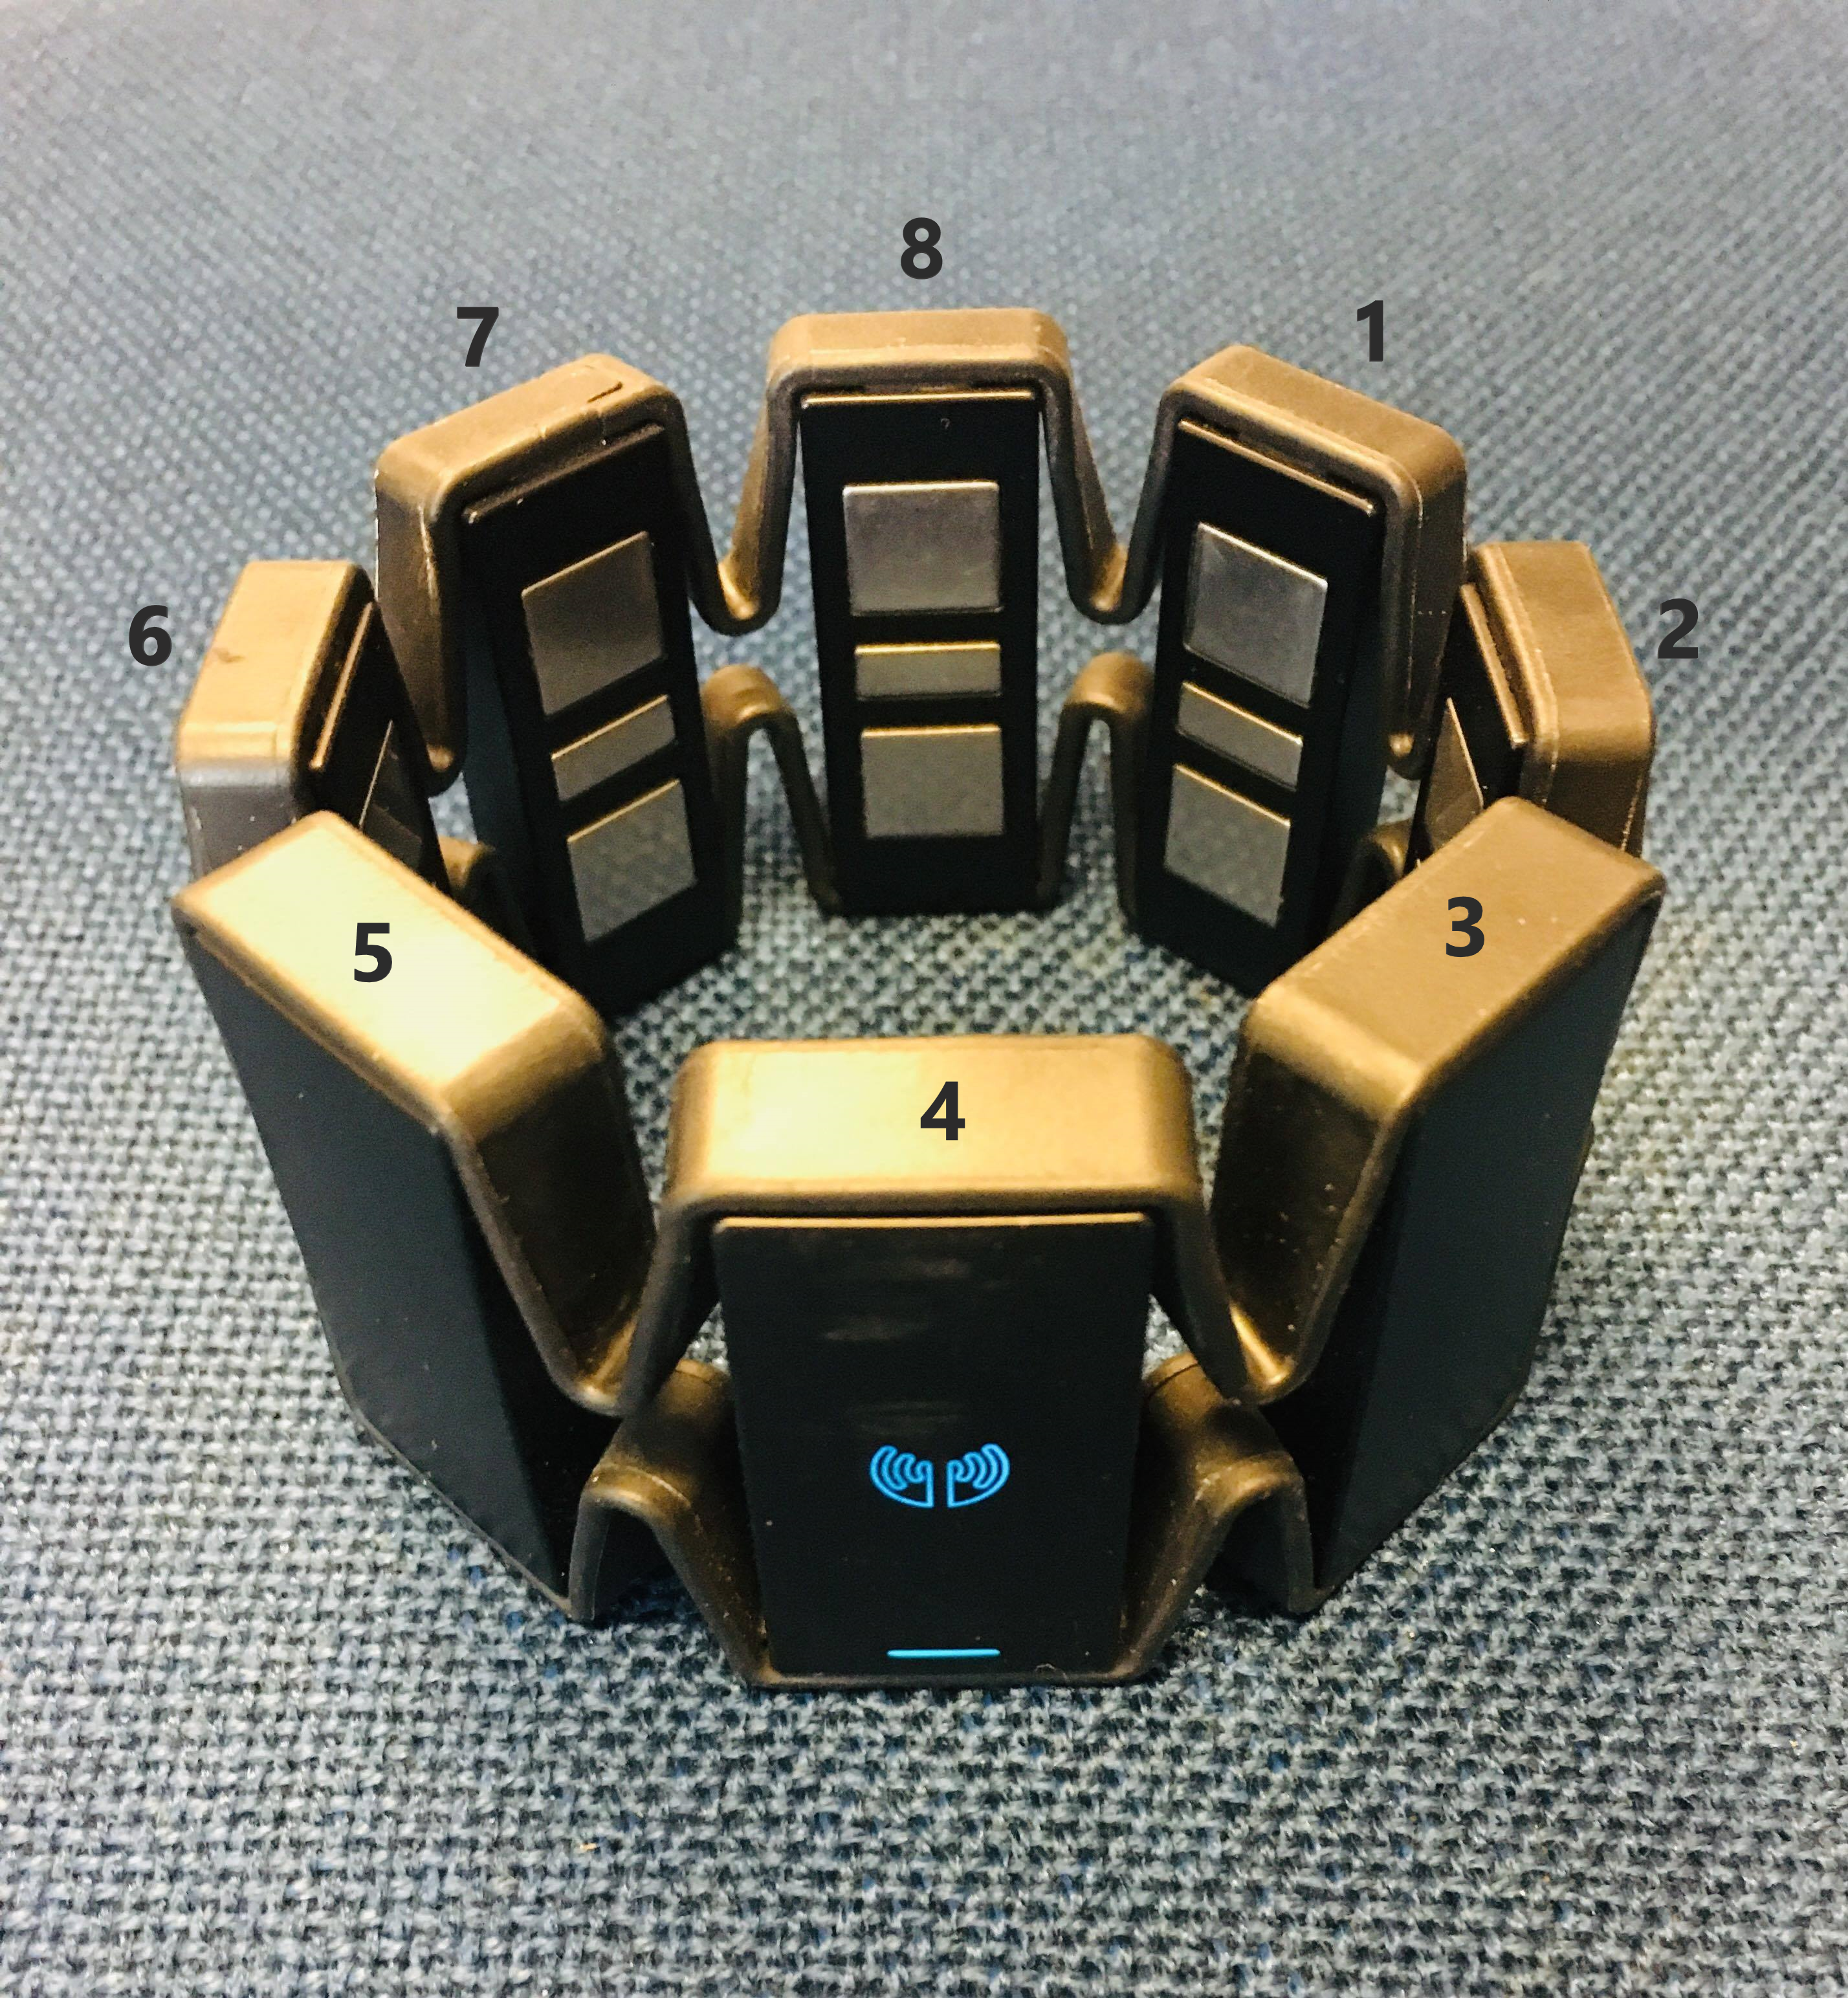
\includegraphics[width=.4\textwidth]{figures/MYB}  
	\caption{Image of the Myo armband from Thalmic Labs. Electrode channel 1 corresponds to the first output in the recording and electrode channel 2 as the second etc., as seen in \figref{fig:Emg_rot}.}
	\label{fig:MYB} 
\end{figure}